\section{x86}

\subsection{\IFRU{Терминология}{Terminology}}

\IFRU{Общее для}{Common for} 16-bit (8086/80286), 32-bit (80386, \IFRU{и т.д.}{etc}), 64-bit.

\index{IEEE 754}
\begin{description}
	\item[byte] 8-bit. \IFRU{Для определения массива байт используется директива ассемблера DB}
		{DB assembly directive is used for defining array of bytes}.
	\item[word] 16-bit. \IFRU{\dittoclosing{} директива ассемблера DW}
		{DW assembly directive \dittoclosing{}}.
	\item[double word] (``dword'') 32-bit. \IFRU{\dittoclosing{} директива ассемблера DD}
		{DD assembly directive \dittoclosing{}}.
	\item[quad word] (``qword'') 64-bit. \IFRU{\dittoclosing{} директива ассемблера DQ}
		{DQ assembly directive \dittoclosing{}}.
	\item[tbyte] (\IFRU{10 байт}{ten bytes}) 80-bit \OrENRU 10 \IFRU{байт}{bytes} 
		(\IFRU{используется для регистров}{used for} IEEE 754 FPU\IFRU{}{ registers}).
\end{description}

\index{Windows API}
\IFRU{Точно такие же типы данных используются и в}
{These data types are also the same as in} Windows \ac{API}.

\section{\IFRU{Регистры общего пользования}{General purpose registers}}

\IFRU{Ко многим регистрам можно обращаться как к частям размером в байт или 16-битное слово}
{It is possible to access many registers by byte or 16-bit word parts}.
\IFRU{Это всё\EMDASH{}наследие от более старых процессоров Intel (вплоть до 8-битного 8080),
все еще поддерживаемое для обратной совместимости}{It is all inheritance from older Intel CPUs (up to 8-bit 8080) 
still supported for backward compatibility}.
\IFRU{Например, в \ac{RISC} процессорах, такой возможности, как правило, нет}{For example, this feature
is usually not present in \ac{RISC} CPUs}.

\index{x86-64}
\IFRU{Регистры, имеющие префикс R- появились только в x86-64, а префикс E- ~--- в 80386}
{Registers prefixed with R- appeared in x86-84, and those prefixed with E-~---in 80386}.
\IFRU{Таким образом, R-регистры 64-битные, а E-регистры ~--- 32-битные}
{Thus, R-registers are 64-bit, and E-registers~---32-bit}.

\IFRU{В x86-64 добавили еще 8 \ac{GPR}: R8-R15}
{8 more \ac{GPR}'s were added in x86-86: R8-R15}.

N.B.: \IFRU{В документации от Intel, для обращения к самому младшему байту к имени регистра
нужно добавлять суффикс \IT{L}: \IT{R8L}, но \ac{IDA} называет эти регистры добавляя суффикс \IT{B}: \IT{R8B}}
{In the Intel manuals byte parts of these registers are prefixed by \IT{L}, e.g.: \IT{R8L}, but \ac{IDA}
names these registers by adding \IT{B} suffix, e.g.: \IT{R8B}}.

\subsection{RAX/EAX/AX/AL}
\RegTableOne{RAX}{EAX}{AX}{AH}{AL}

\ac{AKA} \IFRU{аккумулятор}{accumulator}.
\IFRU{Результат ф-ции обычно возвращается через этот регистр}
{The result of function if usually returned via this register}.

\subsection{RBX/EBX/BX/BL}
\RegTableOne{RBX}{EBX}{BX}{BH}{BL}

\subsection{RCX/ECX/CX/CL}
\RegTableOne{RCX}{ECX}{CX}{CH}{CL}

\ac{AKA} \IFRU{счетчик}{counter}: 
\IFRU{используется в этой роли в инструкциях с префиксом REP и в инструкциях сдвига}
{in this role it is used in REP prefixed instructions and also in shift instructions}
(SHL/SHR/RxL/RxR).

\subsection{RDX/EDX/DX/DL}
\RegTableOne{RDX}{EDX}{DX}{DH}{DL}

\subsection{RSI/ESI/SI/SIL}
\RegTableTwo{RSI}{ESI}{SI}{SIL}

\ac{AKA} ``source''. \IFRU{Используется как источник в инструкциях}{Used as source in the instructions} 
REP MOVSx, REP CMPSx.

\subsection{RDI/EDI/DI/DIL}
\RegTableTwo{RDI}{EDI}{DI}{DIL}

\ac{AKA} ``destination''. \IFRU{Используется как указатель на место назначения в инструкции}
{Used as a pointer to destination place in the instructions} REP MOVSx, REP STOSx.

\subsection{R8/R8D/R8W/R8L}
\RegTableThree{R8}{R8D}{R8W}{R8L}

\subsection{R9/R9D/R9W/R9L}
\RegTableThree{R9}{R9D}{R9W}{R9L}

\subsection{R10/R10D/R10W/R10L}
\RegTableThree{R10}{R10D}{R10W}{R10L}

\subsection{R11/R11D/R11W/R11L}
\RegTableThree{R11}{R11D}{R11W}{R11L}

\subsection{R12/R12D/R12W/R12L}
\RegTableThree{R12}{R12D}{R12W}{R12L}

\subsection{R13/R13D/R13W/R13L}
\RegTableThree{R13}{R13D}{R13W}{R13L}

\subsection{R14/R14D/R14W/R14L}
\RegTableThree{R14}{R14D}{R14W}{R14L}

\subsection{R15/R15D/R15W/R15L}
\RegTableThree{R15}{R15D}{R15W}{R15L}

\subsection{RSP/ESP/SP/SPL}
\RegTableTwo{RSP}{ESP}{SP}{SPL}

\ac{AKA} \gls{stack pointer}. \IFRU{Обычно всегда указывает на текущий стек, кроме тех случаев,
когда он не инициализирован}{Usually points to the current stack except those cases when it is not yet initialized}.

\subsection{RBP/EBP/BP/BPL}
\RegTableTwo{RBP}{EBP}{BP}{BPL}

\ac{AKA} frame pointer. \IFRU{Обычно используется для доступа к локальным переменным ф-ции и аргументам,
Больше о нем}
{Usually used for local variables and arguments of function accessing. More about it}: (\ref{stack_frame}).

\subsection{RIP/EIP/IP}

\begin{center}
\begin{tabular}{ | l | l | l | l | l | l | l | l | l |}
\hline
\RegHeader \\
\hline
\multicolumn{8}{ | c | }{RIP\textsuperscript{x64}} \\
\hline
\multicolumn{4}{ | c | }{} & \multicolumn{4}{ c | }{EIP} \\
\hline
\multicolumn{6}{ | c | }{} & \multicolumn{2}{ c | }{IP} \\
\hline
\end{tabular}
\end{center}

\ac{AKA} ``instruction pointer''
\footnote{\IFRU{Иногда называется так же}{Sometimes also called} ``program counter''}.
\IFRU{Обычно всегда указывает на исполняющуюся инструкцию}{Usually always points to the current instruction}.
\IFRU{Напрямую модифицировать
регистр нельзя, хотя можно делать так (что равноценно)}
{Cannot be modified, however, it is possible to do (which is equivalent to)}:

\begin{lstlisting}
mov eax...
jmp eax
\end{lstlisting}

\IFRU{Либо}{Or}:

\begin{lstlisting}
push val
ret
\end{lstlisting}

\subsection{CS/DS/ES/SS/FS/GS}

\IFRU{16-битные регистры, содержащие селектор кода}{16-bit registers containing code selector} (CS), 
\IFRU{данных}{data selector} (DS), \IFRU{стека}{stack selector} (SS).\\
\\
\index{TLS}
\index{Windows!TIB}
FS \InENRU win32 \IFRU{указывает на}{points to} \ac{TLS}, \IFRU{а в Linux на эту роль был выбран GS}
{GS took this role in Linux}.
\IFRU{Это сделано для более быстрого доступа к \ac{TLS} и прочим структурам там вроде \ac{TIB}}
{It is done for faster access to the \ac{TLS} and other structures like \ac{TIB}}.
\\
\IFRU{В прошлом эти регистры использовались как сегментные регистры}
{In the past, these registers were used as segment registers} (\ref{8086_memory_model}).

\subsection{\IFRU{Регистр флагов}{Flags register}}

\label{EFLAGS}
\ac{AKA} EFLAGS.

\begin{center}
\begin{tabular}{ | l | l | l | }
\hline
\headercolor{} \IFRU{Бит}{Bit} (\IFRU{маска}{mask}) &
\headercolor{} \IFRU{Аббревиатура}{Abbreviation} (\IFRU{значение}{meaning}) &
\headercolor{} \IFRU{Описание}{Description} \\
\hline
0 (1) & CF (Carry) & \RU{Флаг переноса.} \\
      &            & \IFRU{Инструкции}{The} CLC/STC/CMC \IFRU{используются}{instructions are used} \\
      &            & \IFRU{для установки/сброса/инвертирования этого флага}{for setting/resetting/toggling this flag} \\
\hline
2 (4) & PF (Parity) & \RU{Флаг четности }(\ref{parity_flag}). \\
\hline
4 (0x10) & AF (Adjust) & \\
\hline
6 (0x40) & ZF (Zero) & \IFRU{Выставляется в}{Setting to} 0 \\
         &           & \IFRU{если результат последней операции был}{if the last operation's result was} 0. \\
\hline
7 (0x80) & SF (Sign) & \RU{Флаг знака.} \\
\hline
8 (0x100) & TF (Trap) & \IFRU{Применяется при отладке}{Used for debugging}. \\
&         &             \IFRU{Если включен, то после исполнения каждой инструкции}{If turned on, an exception will be} \\
&         &             \IFRU{будет сгенерировано исключение}{generated after each instruction execution}. \\
\hline
9 (0x200) & IF (Interrupt enable) & \IFRU{Разрешены ли прерывания}{Are interrupts enabled}. \\
          &                       & \IFRU{Инструкции}{The} CLI/STI \IFRU{используются}{instructions are used} \\
	  &                       & \IFRU{для установки/сброса этого флага}{for the flag setting/resetting} \\
\hline
10 (0x400) & DF (Direction) & \IFRU{Задается направление для инструкций}{A directions is set for the} \\
           &                & REP MOVSx, REP CMPSx, REP LODSx, REP SCASx\EN{ instructions}.\\
           &                & \IFRU{Инструкции}{The} CLD/STD \IFRU{используются}{instructions are used} \\
	   &                & \IFRU{для установки/сброса этого флага}{for the flag setting/resetting} \\
\hline
11 (0x800) & OF (Overflow) & \RU{Переполнение.} \\
\hline
12, 13 (0x3000) & IOPL (I/O privilege level)\textsuperscript{80286} & \\
\hline
14 (0x4000) & NT (Nested task)\textsuperscript{80286} & \\
\hline
16 (0x10000) & RF (Resume)\textsuperscript{80386} & \IFRU{Применяется при отладке}{Used for debugging}. \\
             &                  & \IFRU{Если включить,}{CPU will ignore hardware breakpoint in DRx} \\
	     &                  & \IFRU{CPU проигнорирует хардварную точку останова в DRx}{if the flag is set}. \\
\hline
17 (0x20000) & VM (Virtual 8086 mode)\textsuperscript{80386} & \\
\hline
18 (0x40000) & AC (Alignment check)\textsuperscript{80486} & \\
\hline
19 (0x80000) & VIF (Virtual interrupt)\textsuperscript{Pentium} & \\
\hline
20 (0x100000) & VIP (Virtual interrupt pending)\textsuperscript{Pentium} & \\
\hline
21 (0x200000) & ID (Identification)\textsuperscript{Pentium} & \\
\hline
\end{tabular}
\end{center}

\IFRU{Остальные флаги зарезервированы}{All the rest flags are reserved}.

\section{FPU-\IFRU{регистры}{registers}}

\index{x86!FPU}
8 80-\IFRU{битных регистров работающих как стек}{bit registers working as a stack}: ST(0)-ST(7).
N.B.: \ac{IDA} \IFRU{называет}{calls} ST(0) \IFRU{просто}{as just} ST.
\IFRU{Числа хранятся в формате}{Numbers are stored in the} IEEE 754\EN{ format}.

\IFRU{Формат значения \IT{long double}}{\IT{long double} value format}:

\bigskip
% a hack used here! http://tex.stackexchange.com/questions/73524/bytefield-package
\begin{center}
\begingroup
\makeatletter
\let\saved@bf@bitformatting\bf@bitformatting
\renewcommand*{\bf@bitformatting}{%
	\ifnum\value{header@val}=21 %
	\value{header@val}=62 %
	\else\ifnum\value{header@val}=22 %
	\value{header@val}=63 %
	\else\ifnum\value{header@val}=23 %
	\value{header@val}=64 %
	\else\ifnum\value{header@val}=30 %
	\value{header@val}=78 %
	\else\ifnum\value{header@val}=31 %
	\value{header@val}=79 %
	\fi\fi\fi\fi\fi
	\saved@bf@bitformatting
}%
\begin{bytefield}{32}
	\bitheader[endianness=big]{0,21,22,23,30,31} \\
	\bitbox{1}{S} &
	\bitbox{8}{\IFRU{экспонента}{exponent}} &
	\bitbox{1}{I} &
	\bitbox{22}{\IFRU{мантисса}{mantissa or fraction}}
\end{bytefield}
\endgroup
\end{center}

\begin{center}
( S\EMDASH{}\IFRU{знак}{sign}, I\EMDASH{}\IFRU{целочисленная часть}{integer part} )
\end{center}

\label{FPU_control_word}
\subsection{\IFRU{Регистр управления}{Control Word}}

\IFRU{Регистр, при помощи которого можно задавать поведение}{Register controlling behaviour of the}
\ac{FPU}.

\begin{center}
\begin{tabular}{ | l | l | l | }
\hline
\IFRU{Бит}{Bit} &
\IFRU{Аббревиатура (значение)}{Abbreviation (meaning)} &
\IFRU{Описание}{Description} \\
\hline
0   & IM (Invalid operation Mask) & \\
\hline
1   & DM (Denormalized operand Mask) & \\
\hline
2   & ZM (Zero divide Mask) & \\
\hline
3   & OM (Overflow Mask) & \\
\hline
4   & UM (Underflow Mask) & \\
\hline
5   & PM (Precision Mask) & \\
\hline
7   & IEM (Interrupt Enable Mask) & \IFRU{Разрешение исключений, по умолчанию 1 (запрещено)}
{Exceptions enabling, 1 by default (disabled)} \\
\hline
8, 9 & PC (Precision Control) & \RU{Управление точностью} \\
     &                        & 00 ~--- 24 \IFRU{бита}{bits} (REAL4) \\
     &                        & 10 ~--- 53 \IFRU{бита}{bits} (REAL8) \\
     &                        & 11 ~--- 64 \IFRU{бита}{bits} (REAL10) \\
\hline
10, 11 & RC (Rounding Control) & \RU{Управление округлением} \\
       &                       & 00 ~--- \IFRU{(по умолчанию) округлять к ближайшему}{(by default) round to nearest} \\
       &                       & 01 ~--- \IFRU{округлять к}{round toward} $-\infty$ \\
       &                       & 10 ~--- \IFRU{округлять к}{round toward} $+\infty$ \\
       &                       & 11 ~--- \IFRU{округлять к}{round toward} $0$ \\
\hline
12 & IC (Infinity Control) & 0 ~--- (\IFRU{по умолчанию}{by default}) \IFRU{считать}{treat} $+\infty$ \AndENRU $-\infty$ \IFRU{за беззнаковое}{as unsigned} \\
   &                       & 1 ~--- \IFRU{учитывать и}{respect both} $+\infty$ \AndENRU $-\infty$ \\
\hline
\end{tabular}
\end{center}

\IFRU{Флагами}{The} PM, UM, OM, ZM, DM, IM 
\IFRU{задается, генерировать ли исключения в случае соответствующих ошибок}
{flags are defining if to generate exception in case of corresponding errors}.

\subsection{\IFRU{Регистр статуса}{Status Word}}

\label{FPU_status_word}
\IFRU{Регистр только для чтения}{Read-only register}.

\begin{center}
\begin{tabular}{ | l | l | l | }
\hline
\IFRU{Бит}{Bit} &
\IFRU{Аббревиатура (значение)}{Abbreviation (meaning)} &
\IFRU{Описание}{Description} \\
\hline
15   & B (Busy) & \IFRU{Работает ли сейчас FPU}{Is FPU do something} (1)
\IFRU{или закончил и результаты готовы}{or results are ready} (0) \\
\hline
14   & C3 & \\
\hline
13, 12, 11 & TOP & \IFRU{указывает, какой сейчас регистр является нулевым}
{points to the currently zeroth register} \\
\hline
10 & C2 & \\
\hline
9  & C1 & \\
\hline
8  & C0 & \\
\hline
7  & IR (Interrupt Request) & \\
\hline
6  & SF (Stack Fault) & \\
\hline
5  & P (Precision) & \\
\hline
4  & U (Underflow) & \\
\hline
3  & O (Overflow) & \\
\hline
2  & Z (Zero) & \\
\hline
1  & D (Denormalized) & \\
\hline
0  & I (Invalid operation) & \\
\hline
\end{tabular}
\end{center}

\IFRU{Биты}{The} SF, P, U, O, Z, D, I \IFRU{сигнализируют об исключениях}
{bits are signaling about exceptions}.

\IFRU{О}{About the} C3, C2, C1, C0 \IFRU{читайте больше}{read more}: (\ref{Czero_etc}).

N.B.: \IFRU{когда используется регистр ST(x), FPU прибавляет $x$ к TOP по модулю 8 и получается номер
внутреннего регистра}{When ST(x) is used, FPU adds $x$ to TOP (by modulo 8) and that is how it gets 
internal register's number}.

\subsection{Tag Word}

\IFRU{Этот регистр отражает текущее содержимое регистров чисел}
{The register has current information about number's registers usage}.

\begin{center}
\begin{tabular}{ | l | l | l | }
\hline
\IFRU{Бит}{Bit} & \IFRU{Аббревиатура (значение)}{Abbreviation (meaning)} \\
\hline
15, 14 & Tag(7) \\
\hline
13, 12 & Tag(6) \\
\hline
11, 10 & Tag(5) \\
\hline
9, 8 & Tag(4) \\
\hline
7, 6 & Tag(3) \\
\hline
5, 4 & Tag(2) \\
\hline
3, 2 & Tag(1) \\
\hline
1, 0 & Tag(0) \\
\hline
\end{tabular}
\end{center}

\IFRU{Для каждого тэга}{For each tag}:

\begin{itemize}
\item
00 ~--- \IFRU{Регистр содержит ненулевое значение}{The register contains a non-zero value}
\item
01 ~--- \IFRU{Регистр содержит 0}{The register contains 0}
\item
10 ~--- \IFRU{Регистр содержит специальное число}{The register contains a special value} 
(\ac{NAN}, $\infty$, \OrENRU \IFRU{денормализованное число}{denormal})
\item
11 ~--- \IFRU{Регистр пуст}{The register is empty}
\end{itemize}

\section{SIMD-\IFRU{регистры}{registers}}

\subsection{MMX-\IFRU{регистры}{registers}}

8 64-\IFRU{битных регистров}{bit registers}: MM0..MM7.

\subsection{SSE \AndENRU AVX-\IFRU{регистры}{registers}}

\index{x86-64}
SSE: 8 128-\IFRU{битных регистров}{bit registers}: XMM0..XMM7.
\IFRU{В}{In the} x86-64 \IFRU{добавлено еще 8 регистров}{8 more registers were added}: XMM8..XMM15.

AVX \IFRU{это расширение всех регистры до 256 бит}{is the extension of all these registers to 256 bits}.

\subsection{\RU{Отладочные регистры}\EN{Debugging registers}}

\RU{Применяются для работы с т.н.}\EN{Used for} hardware breakpoints\EN{ control}.

\begin{itemize}
	\item DR0 --- \RU{адрес точки останова}\EN{address of breakpoint} \#1
	\item DR1 --- \RU{адрес точки останова}\EN{address of breakpoint} \#2
	\item DR2 --- \RU{адрес точки останова}\EN{address of breakpoint} \#3
	\item DR3 --- \RU{адрес точки останова}\EN{address of breakpoint} \#4
	\item DR6 --- \RU{здесь отображается причина останова}\EN{a cause of break is reflected here}
	\item DR7 --- \RU{здесь можно задать типы точек останова}\EN{breakpoint types are set here}
\end{itemize}

\subsubsection{DR6}
\myindex{x86!\Registers!DR6}

\begin{center}
\begin{tabular}{ | l | l | }
\hline
\headercolor\ \RU{Бит}\EN{Bit} (\RU{маска}\EN{mask}) &
\headercolor\ \RU{Описание}\EN{Description} \\
\hline
0 (1)       &  B0 --- \RU{сработала точка останова \#1}\EN{breakpoint \#1 has been triggered} \\
\hline
1 (2)       &  B1 --- \RU{сработала точка останова \#2}\EN{breakpoint \#2 has been triggered} \\
\hline
2 (4)       &  B2 --- \RU{сработала точка останова \#3}\EN{breakpoint \#3 has been triggered} \\
\hline
3 (8)       &  B3 --- \RU{сработала точка останова \#4}\EN{breakpoint \#4 has been triggered} \\
\hline
13 (0x2000) &  BD --- \RU{была попытка модифицировать один из регистров DRx.}
               \EN{modification attempt of one of the DRx registers.} \\
            &  \RU{может быть выставлен если бит GD выставлен.}
	       \EN{may be raised if GD is enabled} \\
\hline
14 (0x4000) &  BS --- \RU{точка останова типа single step (флаг TF был выставлен в EFLAGS)}
               \EN{single step breakpoint (TF flag has been set in EFLAGS)}. \\
	    &  \RU{Наивысший приоритет. Другие биты также могут быть выставлены}
	       \EN{Highest priority. Other bits may also be set}. \\
\hline
% TODO: describe BT
15 (0x8000) &  BT (task switch flag) \\
\hline
\end{tabular}
\end{center}

N.B. \RU{Точка останова single step это срабатывающая после каждой инструкции}
\EN{A single step breakpoint is a breakpoint which occurs after each instruction}.
\RU{Может быть включена выставлением флага TF в EFLAGS}
\EN{It can be enabled by setting TF in EFLAGS} (\myref{EFLAGS}).

\subsubsection{DR7}
\myindex{x86!\Registers!DR7}

\RU{В этом регистре задаются типы точек останова}\EN{Breakpoint types are set here}.

\small
\begin{center}
\begin{tabular}{ | l | l | }
\hline
\headercolor\ \RU{Бит}\EN{Bit} (\RU{маска}\EN{mask}) &
\headercolor\ \RU{Описание}\EN{Description} \\
\hline
0 (1)       &  L0 --- \RU{разрешить точку останова}\EN{enable breakpoint} \#1 \RU{для текущей задачи}\EN{for the current task} \\
\hline
1 (2)       &  G0 --- \RU{разрешить точку останова}\EN{enable breakpoint} \#1 \RU{для всех задач}\EN{for all tasks} \\
\hline
2 (4)       &  L1 --- \RU{разрешить точку останова}\EN{enable breakpoint} \#2 \RU{для текущей задачи}\EN{for the current task} \\
\hline
3 (8)       &  G1 --- \RU{разрешить точку останова}\EN{enable breakpoint} \#2 \RU{для всех задач}\EN{for all tasks} \\
\hline
4 (0x10)    &  L2 --- \RU{разрешить точку останова}\EN{enable breakpoint} \#3 \RU{для текущей задачи}\EN{for the current task} \\
\hline
5 (0x20)    &  G2 --- \RU{разрешить точку останова}\EN{enable breakpoint} \#3 \RU{для всех задач}\EN{for all tasks} \\
\hline
6 (0x40)    &  L3 --- \RU{разрешить точку останова}\EN{enable breakpoint} \#4 \RU{для текущей задачи}\EN{for the current task} \\
\hline
7 (0x80)    &  G3 --- \RU{разрешить точку останова}\EN{enable breakpoint} \#4 \RU{для всех задач}\EN{for all tasks} \\
\hline
8 (0x100)   &  LE --- \RU{не поддерживается, начиная с P6}\EN{not supported since P6} \\
\hline
9 (0x200)   &  GE --- \RU{не поддерживается, начиная с P6}\EN{not supported since P6} \\
\hline
13 (0x2000) &  GD --- \RU{исключение будет вызвано если какая-либо инструкция MOV}
			\EN{exception is to be raised if any MOV instruction} \\
            & \RU{попытается модифицировать один из DRx-регистров}
			\EN{tries to modify one of the DRx registers} \\
\hline
16,17 (0x30000)    &  \RU{точка останова}\EN{breakpoint} \#1: R/W --- \RU{тип}\EN{type} \\
\hline
18,19 (0xC0000)    &  \RU{точка останова}\EN{breakpoint} \#1: LEN --- \RU{длина}\EN{length} \\
\hline
20,21 (0x300000)   &  \RU{точка останова}\EN{breakpoint} \#2: R/W --- \RU{тип}\EN{type} \\
\hline
22,23 (0xC00000)   &  \RU{точка останова}\EN{breakpoint} \#2: LEN --- \RU{длина}\EN{length} \\
\hline
24,25 (0x3000000)  &  \RU{точка останова}\EN{breakpoint} \#3: R/W --- \RU{тип}\EN{type} \\
\hline
26,27 (0xC000000)  &  \RU{точка останова}\EN{breakpoint} \#3: LEN --- \RU{длина}\EN{length} \\
\hline
28,29 (0x30000000) &  \RU{точка останова}\EN{breakpoint} \#4: R/W --- \RU{тип}\EN{type} \\
\hline
30,31 (0xC0000000) &  \RU{точка останова}\EN{breakpoint} \#4: LEN --- \RU{длина}\EN{length} \\
\hline
\end{tabular}
\end{center}
\normalsize

\RU{Так задается тип точки останова}\EN{The breakpoint type is to be set as follows} (R/W):

\begin{itemize}
\item 00 --- \RU{исполнение инструкции}\EN{instruction execution}
\item 01 --- \RU{запись в память}\EN{data writes}
\item 10 --- \RU{обращения к I/O-портам (недоступно из user-mode)}\EN{I/O reads or writes (not available in user-mode)}
\item 11 --- \RU{обращение к памяти (чтение или запись)}\EN{on data reads or writes}
\end{itemize}

N.B.: \RU{отдельного типа для чтения из памяти действительно нет}
\EN{breakpoint type for data reads is absent, indeed}. \\
\\
\RU{Так задается длина точки останова}\EN{Breakpoint length is to be set as follows} (LEN):

\begin{itemize}
\item 00 --- \RU{1 байт}\EN{one-byte}
\item 01 --- \RU{2 байта}\EN{two-byte}
\item 10 --- \RU{не определено для 32-битного режима, 8 байт для 64-битного}
		\EN{undefined for 32-bit mode, eight-byte in 64-bit mode}
\item 11 --- \RU{4 байта}\EN{four-byte}
\end{itemize}


% TODO: control registers
 % subsection
% to be proofreaded
\subsection{\IFRU{Инструкции}{Instructions}}

\IFRU{Инструкции отмеченные как (M) обычно не генерируются компилятором: если вы видите её, вероятно,
это вручную написанный фрагмент кода, либо это т.н. compiler intrinsic}
{Instructions marked as (M) are not usually generated by compiler: if you see it, it is probably
hand-written piece of assembly code, or this is compiler intrinsic} (\ref{compiler_intrinsic}).

% TODO ? обратные инструкции

\IFRU{Только наиболее используемые инструкции перечислены здесь}
{Only most frequently used instructions are listed here}.
\IFRU{Обращайтесь к}{Read} \cite{Intel} \OrENRU \cite{AMD} 
\IFRU{для полной документации}{for a full documentation}.

\subsubsection{\IFRU{Префиксы}{Prefixes}}

\begin{description}
\label{x86_lock}
\item[LOCK] \IFRU{используется чтобы предоставить эксклюзивный доступ к памяти в многопроцессорной среде}
{force CPU to make exclusive access to the RAM in multiprocessor environment}.
\IFRU{Для упрощения, можно сказать, что когда исполняется инструкция с этим префиксом, остальные процессоры
в системе останавливаются}{For the sake of simplification, it can be said that when instruction
with this prefix is executed, all other CPUs in multiprocessor system is stopped}.
\IFRU{Чаще все это используется для критических секций, семафоров, мьютексов}{Most often
it is used for critical sections, semaphores, mutexes}.
\IFRU{Обычно используется с}{Commonly used with} ADD, AND, BTR, BTS, CMPXCHG, OR, XADD, XOR.
\IFRU{Читайте больше о критических секциях}{Read more about critical sections} (\ref{critical_sections}).

\item[REP] \IFRU{используется с инструкциями}{used with} MOVSx \AndENRU STOSx\IFRU{ instructions}{}:
\IFRU{инструкция будет исполняться в цикле, счетчик расположен в регистре CX/ECX/RCX}
{execute the instruction in loop, counter is located in the CX/ECX/RCX register}.
\IFRU{Для более детального описания, читайте больше об инструкциях}
{For detailed description, read more about} MOVSx (\ref{REP_MOVSx}) 
\AndENRU STOSx (\ref{REP_STOSx})\IFRU{}{ instructions}.

\IFRU{Работа инструкций с префиксом REP зависит от флага DF, он задает направление}
{Instructions prefixed by REP are sensitive to DF flag, which is used to set direction}.

\item[REPE/REPNE] (\ac{AKA} REPZ/REPNZ) \IFRU{используется с инструкциями}{used with} CMPSx \AndENRU
SCASx\IFRU{ instructions}{}:
\IFRU{инструкция будет исполняться в цикле, счетчик расположен в регистре CX/ECX/RCX}
{execute the last instruction in loop, count is set in the CX/ECX/RCX register}. 
\IFRU{Выполнение будет прервано если ZF будет 0 (REPE) либо если ZF будет 1 (REPNE)}
{It will terminate prematurely if ZF is 0 (REPE) or if ZF is 1 (REPNE)}.

\IFRU{Для более детального описания, читайте больше об инструкциях}
{For detailed description, read more about} CMPSx (\ref{REPE_CMPSx}) 
\AndENRU SCASx (\ref{REPNE_SCASx})\IFRU{}{ instructions}.

\IFRU{Работа инструкций с префиксами REPE/REPNE зависит от флага DF, он задает направление}
{Instructions prefixed by REPE/REPNE are sensitive to DF flag, which is used to set direction}.

\end{description}

\subsubsection{\IFRU{Наиболее часто используемые инструкции}{Most frequently used instructions}}

\IFRU{Их можно заучить в первую очередь}{These can be memorized in the first place}.

\begin{description}
% in order to keep them easily sorted...
\myindex{x86!\Instructions!ADC}
\myindex{x86!\Flags!CF}
  \item[ADC] (\IT{add with carry}) \RU{сложить два значения, \glslink{increment}{инкремент} 
  если выставлен флаг CF.
  ADC часто используется для складывания больших значений, например, складывания двух 64-битных
  значений в 32-битной среде используя две инструкции ADD и ADC, например:}
  \EN{add values, \gls{increment} the result if the CF flag is set.
  ADC is often used for the addition of large values, for example, 
  to add two 64-bit values in a 32-bit environment using two ADD and ADC instructions. For example:}

\EN{\lstinputlisting{appendix/x86/instructions/ADC_example_EN.lst}}
\RU{\lstinputlisting{appendix/x86/instructions/ADC_example_RU.lst}}

\RU{Еще один пример}\EN{One more example}: \myref{sec:64bit_in_32_env}.

\index{x86!\Instructions!ADD}
  \item[ADD] \IFRU{сложить два значения}{add two values}

\myindex{x86!\Instructions!AND}
  \item[AND] \RU{логическое \q{И}}\EN{logical \q{and}}

\index{x86!\Instructions!CALL}
  \item[CALL] \RU{вызвать другую ф-цию}\EN{call another function}: \TT{PUSH address\_after\_CALL\_instruction; JMP label}

\index{x86!\Instructions!CMP}
  \item[CMP] \IFRU{сравнение значений и установка флагов, то же что и \TT{SUB}, но только без записи результата}
  {compare values and set flags, the same as \TT{SUB} but no results writing}

\myindex{x86!\Instructions!DEC}
\myindex{x86!\Flags!CF}
  \item[DEC] \gls{decrement}.%
\RU{В отличие от других арифметических инструкций, \TT{INC} не модифицирует флаг CF.}%
\EN{Unlike other arithmetic instructions, \TT{INC} doesn't modify CF flag.}


\myindex{x86!\Instructions!IMUL} 
  \item[IMUL] \RU{умножение с учетом знаковых значений}\EN{signed multiply}
  \EN{\IMUL often used instead of \MUL, read more about it: \ref{IMUL_over_MUL}.}
% TODO translate


\myindex{x86!\Instructions!INC} 
\myindex{x86!\Flags!CF}
  \item[INC] \gls{increment}.%
\RU{В отличие от других арифметических инструкций, \TT{INC} не модифицирует флаг CF.}%
\EN{Unlike other arithmetic instructions, \TT{INC} doesn't modify CF flag.}

\myindex{x86!\Instructions!JCXZ}
\myindex{x86!\Instructions!JECXZ}
\myindex{x86!\Instructions!JRCXZ}
  \item[JCXZ, JECXZ, JRCXZ] (M) \RU{переход если CX/ECX/RCX=0}\EN{jump if CX/ECX/RCX=0}

\index{x86!\Instructions!JMP}
  \item[JMP] \IFRU{перейти на другой адрес}{jump to another address}

\item[Jcc] (\IFRU{где}{where} cc\EMDASH{}condition code)

\index{x86!\Instructions!JAE}
\index{x86!\Instructions!JA}
\index{x86!\Instructions!JBE}
\index{x86!\Instructions!JB}
\index{x86!\Instructions!JC}
\index{x86!\Instructions!JE}
\index{x86!\Instructions!JGE}
\index{x86!\Instructions!JG}
\index{x86!\Instructions!JLE}
\index{x86!\Instructions!JL}
\index{x86!\Instructions!JNAE}
\index{x86!\Instructions!JNA}
\index{x86!\Instructions!JNBE}
\index{x86!\Instructions!JNB}
\index{x86!\Instructions!JNC}
\index{x86!\Instructions!JNE}
\index{x86!\Instructions!JNGE}
\index{x86!\Instructions!JNG}
\index{x86!\Instructions!JNLE}
\index{x86!\Instructions!JNL}
\index{x86!\Instructions!JNO}
\index{x86!\Instructions!JNS}
\index{x86!\Instructions!JNZ}
\index{x86!\Instructions!JO}
\index{x86!\Instructions!JPO}
\index{x86!\Instructions!JP}
\index{x86!\Instructions!JS}
\index{x86!\Instructions!JZ}

\IFRU{Немало этих инструкций имеют синонимы (отмечены с AKA), это сделано для удобства}
{A lot of instructions has synonyms (denoted with AKA), this was done for convenience}.
\IFRU{Синонимичные инструкции транслируются в один и тот же опкод}
{Synonymous instructions are translating into the same opcode}.
\IFRU{Опкод имеет т.н.}{Opcode has} \gls{jump offset}.

\label{Jcc}
\begin{description}
\item[JAE] \ac{AKA} JNC: \IFRU{переход если больше или равно (беззнаковый)}{jump if above or equal (unsigned)}: CF=0
\item[JA] \ac{AKA} JNBE: \IFRU{переход если больше (беззнаковый)}{jump if greater (unsigned)}: CF=0 \AndENRU ZF=0
\item[JBE] \IFRU{переход если меньше или равно (беззнаковый)}{jump if lesser or equal (unsigned)}: CF=1 \OrENRU ZF=1
\item[JB] \ac{AKA} JC: \IFRU{переход если меньше (беззнаковый)}{jump if below (unsigned)}: CF=1
\item[JC] \ac{AKA} JB: \IFRU{переход если CF=1}{jump if CF=1}
\item[JE] \ac{AKA} JZ: \IFRU{переход если равно или ноль}{jump if equal or zero}: ZF=1
\item[JGE] \IFRU{переход если больше или равно (знаковый)}{jump if greater or equal (signed)}: SF=OF
\item[JG] \IFRU{переход если больше (знаковый)}{jump if greater (signed)}: ZF=0 \AndENRU SF=OF
\item[JLE] \IFRU{переход если меньше или равно (знаковый)}{jump if lesser or equal (signed)}: ZF=1 \OrENRU SF$\neq$OF
\item[JL] \IFRU{переход если меньше (знаковый)}{jump if lesser (signed)}: SF$\neq$OF
\item[JNAE] \ac{AKA} JC: \IFRU{переход если не больше или равно (беззнаковый)}{jump if not above or equal (unsigned)} CF=1
\item[JNA] \IFRU{переход если не больше (беззнаковый)}{jump if not above (unsigned)} CF=1 \AndENRU ZF=1
\item[JNBE] \IFRU{переход если не меньше или равно (беззнаковый)}{jump if not below or equal (unsigned)}: CF=0 \AndENRU ZF=0
\item[JNB] \ac{AKA} JNC: \IFRU{переход если не меньше (беззнаковый)}{jump if not below (unsigned)}: CF=0
\item[JNC] \ac{AKA} JAE: \IFRU{переход если CF=0, синонимично}{jump CF=0 synonymous to} JNB.
\item[JNE] \ac{AKA} JNZ: \IFRU{переход если не равно или не ноль}{jump if not equal or not zero}: ZF=0
\item[JNGE] \IFRU{переход если не больше или равно (знаковый)}{jump if not greater or equal (signed)}: SF$\neq$OF
\item[JNG] \IFRU{переход если не больше (знаковый)}{jump if not greater (signed)}: ZF=1 \OrENRU SF$\neq$OF
\item[JNLE] \IFRU{переход если не меньше (знаковый)}{jump if not lesser (signed)}: ZF=0 \AndENRU SF=OF
\item[JNL] \IFRU{переход если не меньше (знаковый)}{jump if not lesser (signed)}: SF=OF
\item[JNO] \IFRU{переход если не переполнение}{jump if not overflow}: OF=0
\item[JNS] \IFRU{переход если флаг SF сброшен}{jump if SF flag is cleared}
\item[JNZ] \ac{AKA} JNE: \IFRU{переход если не равно или не ноль}{jump if not equal or not zero}: ZF=0
\item[JO] \IFRU{переход если переполнение}{jump if overflow}: OF=1
\item[JPO] \IFRU{переход если сброшен флаг PF}{jump if PF flag is cleared}
\item[JP] \ac{AKA} JPE: \IFRU{переход если выставлен флаг PF}{jump if PF flag is set}
\item[JS] \IFRU{переход если выставлен флаг SF}{jump if SF flag is set}
\item[JZ] \ac{AKA} JE: \IFRU{переход если равно или ноль}{jump if equal or zero}: ZF=1
\end{description}


\index{x86!\Instructions!LAHF}
  \item[LAHF] \IFRU{скопировать некоторые биты флагов в AH}{copy some flag bits to AH}

\index{x86!\Instructions!LEA}
\item[LEA] (\IT{Load Effective Address}) \IFRU{сформировать адрес}{form address}

\label{sec:LEA}

\newcommand{\URLAM}{\url{http://en.wikipedia.org/wiki/Addressing_mode}}

% to be proofreaded (begin)
\IFRU{Это инструкция которая задумывалась вовсе не для складывания 
и умножения чисел, 
а для формирования адреса например из указателя на массив и прибавления индекса к нему
\footnote{См. также: \URLAM}.}
{This instruction was intended not for values summing and multiplication 
but for address forming, 
e.g., for forming address of array element by adding array address, element index, with 
multiplication of element size\footnote{See also: \URLAM}.}

\IFRU{Тем не менее, её можно использовать для любых других вычислений}
{But nevertheless, it is can be used for any other calculations}.

\IFRU{\LEA удобна тем, что производимые ею вычисления не модифицируют флаги \ac{CPU}.}
{\LEA is convenient because the computations performing by it is not alter \ac{CPU} flags.}
% to be proofreaded (end)

\begin{lstlisting}
int f(int a, int b)
{
	return a*8+b;
};
\end{lstlisting}

\begin{lstlisting}[caption=MSVC 2010 /Ox]
_a$ = 8							; size = 4
_b$ = 12						; size = 4
_f	PROC
	mov	eax, DWORD PTR _b$[esp-4]
	mov	ecx, DWORD PTR _a$[esp-4]
	lea	eax, DWORD PTR [eax+ecx*8]
	ret	0
_f	ENDP
\end{lstlisting}

\index{Intel C++}
Intel C++ \IFRU{использует LEA даже больше}{uses LEA even more}:

\begin{lstlisting}
int f1(int a)
{
	return a*13;
};
\end{lstlisting}

\begin{lstlisting}[caption=Intel C++ 2011]
_f1	PROC NEAR 
        mov       ecx, DWORD PTR [4+esp]      ; ecx = a
	lea       edx, DWORD PTR [ecx+ecx*8]  ; edx = a*9
	lea       eax, DWORD PTR [edx+ecx*4]  ; eax = a*9 + a*4 = a*13
        ret                                
\end{lstlisting}

\IFRU{Эти две инструкции вместо одной IMUL будут работать быстрее}{These two instructions
instead of one IMUL will perform faster}.


% to be proofreaded
\index{\CStandardLibrary!memcpy()}
\index{x86!\Instructions!MOVSB}
\index{x86!\Instructions!MOVSW}
\index{x86!\Instructions!MOVSD}
\index{x86!\Instructions!MOVSQ}
\item[MOVSB/MOVSW/MOVSD/MOVSQ] 
\RU{скопировать}\EN{copy} \RU{байт}\EN{byte}/
16-\RU{битное слово}\EN{bit word}/
32-\RU{битное слово}\EN{bit word}/
64-\RU{битное слово}\EN{bit word} \RU{на который указывает}\EN{address of which is in the} SI/ESI/RSI 
\RU{куда указывает}\EN{into the place address of which is in the} DI/EDI/RDI.

\label{REP_MOVSx}
\RU{Вместе с префиксом REP, инструкция будет исполняться в цикле, счетчик будет
находится в регистре CX/ECX/RCX}
\EN{Together with REP prefix, it will repeated in loop, count is stored in the CX/ECX/RCX register}:
\RU{это работает как}\EN{it works like} memcpy() \RU{в Си}\EN{in C}.
\RU{Если размер блока известен компилятору на стадии компиляции,
memcpy() часто компилируется в короткий фрагмент кода использующий
REP MOVSx, иногда даже несколько инструкций}
\EN{If block size is known to compiler on compile stage, 
memcpy() is often inlined into short code fragment
using REP MOVSx, sometimes even as several instructions}.

\RU{Эквивалент }memcpy(EDI, ESI, 15)\EN{ equivalent is}:

\lstinputlisting{appendix/x86/instructions/MOVSB_ex1_\LANG.asm}

(\RU{Вероятно, так быстрее чем копировать 15 байт используя просто одну}
\EN{Supposedly, it will work faster then copying 15 bytes using just one} REP MOVSB).


\index{x86!\Instructions!MOVSX}
  \item[MOVSX] \RU{загрузить с расширением знака}\EN{load with sign extension} \RU{см. также}\EN{see also}: (\ref{MOVSX})

\myindex{x86!\Instructions!MOVZX}
  \item[MOVZX] \RU{загрузить и очистить все остальные биты}\EN{load and clear all other bits} \RU{см. также}\EN{see also}: (\myref{movzx})

% to be proofreaded
\index{x86!\Instructions!MOV}
\item[MOV] \IFRU{загрузить значение}{load value}. \IFRU{эта инструкция была названа неудачно 
(данные не перемещаются), 
что является результатом путаницы: 
в других архитектурах эта же инструкция называется ``LOAD'' или что-то в этом роде}
{this instruction was named awry resulting confusion (data are not moved), in other architectures 
the same instructions is usually named ``LOAD'' or something like that}.

\IFRU{Важно: если в 32-битном режиме при помощи MOV записывать младшую 16-байтную часть регистра,
то старшие 16 бит останутся такими же.}
{One important thing: if to set low 16-bit part of 32-bit register in 32-bit mode, high 16 bits
will remain as they were.}
\IFRU{Но если в 64-битном режиме модифицировать 32-битную часть регистра, то старшие 32 бита обнуляются.}
{But if to modify low 32-bit of register in 64-bit mode, high 32 bits of registers will be cleared.}

\IFRU{Вероятно, это сделано для упрощения портирования кода под x86-64.}
{Supposedly, it was done for x86-64 code porting simplification.}
 

\index{x86!\Instructions!MUL}
  \item[MUL] \IFRU{умножение с учетом беззнаковых значений}{unsigned multiply}

\myindex{x86!\Instructions!NEG}
  \item[NEG] \RU{смена знака}\EN{negation}: $op=-op$

\index{x86!\Instructions!NOP}
  \item[NOP] \ac{NOP}. \IFRU{Её опкод 0x90, что на самом деле это холостая инструкция}
  {Opcode is 0x90, so it is in fact mean} 
  \TT{XCHG EAX,EAX}\IFRU{}{ idle instruction}.
  \IFRU{Это значит что в x86 (как и во многих \ac{RISC}) нет отдельной \ac{NOP}-инструкции}
  {This means, x86 do not have dedicated \ac{NOP} instruction (as in many \ac{RISC})}.
  \IFRU{Еще примеры подобных операций}{More examples of such operations}:
  (\ref{sec:npad})

\index{x86!\Instructions!NOT}
  \item[NOT] op1: $op1=\neg{}op1$. \RU{логическое ``НЕ''}\EN{logical inversion}

\index{x86!\Instructions!OR}
  \item[OR] \IFRU{логическое ``ИЛИ''}{logical ``or''}

\index{x86!\Instructions!POP}
\item[POP] \IFRU{взять значение из стека}{get value from the stack}:
\TT{value=SS:[ESP]; ESP=ESP+4 (or 8)}

\index{x86!\Instructions!PUSH}
\item[PUSH] \IFRU{записать значение в стек}{push value to stack}: 
\TT{ESP=ESP-4 (\OrENRU 8); SS:[ESP]=value}

% to be proofreaded
\index{x86!\Instructions!RET}
  \item[RET]: \IFRU{возврат из процедуры}{return from subroutine}: \TT{POP tmp; JMP tmp}.
	  \IFRU{В реальности, RET это макрос ассемблера, в среде Windows и *NIX транслирующийся в RETN 
		  (``return near'') либо, во времена MS-DOS, где память адресовалась немного иначе 
	  	(\ref{dos_memory_model}), в RETF (``return far'').}
	  {
		  In fact, RET is a assembly language macro, in Windows and *NIX environment is translating 
		  into RETN
		  (``return near'') or, in MS-DOS times, where memory was addressed differently 
		  (\ref{dos_memory_model}) into RETF (``return far'').
	  }


\myindex{x86!\Instructions!SAHF}
\myindex{x86!\Registers!AH}

  \item[SAHF] \RU{скопировать биты из AH в флаги CPU}\EN{copy bits from AH to CPU flags}:

\begin{center}
\begin{bytefield}[endianness=big,bitwidth=0.03\linewidth]{8}
\bitheader{7,6,4,2,0} \\
\bitbox{1}{SF} & 
\bitbox{1}{ZF} & 
\bitbox{1}{} & 
\bitbox{1}{AF} & 
\bitbox{1}{} & 
\bitbox{1}{PF} & 
\bitbox{1}{} & 
\bitbox{1}{CF}
\end{bytefield}
\end{center}


\index{x86!\Instructions!SBB}
  \item[SBB] (\IT{subtraction with borrow}) 
  \IFRU{вычесть одно значение из другого, \glslink{decrement}{декремент} результата если флаг CF выставлен.
  часто используется для вычитания больших значений, например, для вычитания двух 64-битных
  значений в 32-битной среде используя инструкции SUB и SBB, например:}
  {subtract values, \gls{decrement} result if CF flag is set.
  often used for subtraction of large values, for example,
  to subtract two 64-bit values in 32-bit environment using two SUB and SBB instructions, for example:}

\lstinputlisting{appendix/x86/instructions/SBB_example_\IFRU{ru}{en}.lst}

\index{\CStandardLibrary!strlen()}
\index{\CStandardLibrary!memchr()}
\index{x86!\Instructions!SCASB}
\index{x86!\Instructions!SCASW}
\index{x86!\Instructions!SCASD}
\index{x86!\Instructions!SCASQ}
\item[SCASB/SCASW/SCASD/SCASQ] (M) \RU{сравнить}\EN{compare} \RU{байт}\EN{byte}/
16-\RU{битное слово}\EN{bit word}/
32-\RU{битное слово}\EN{bit word}/
64-\RU{битное слово,}\EN{bit word} \RU{записанное в}\EN{that's stored in}
AX/EAX/RAX \RU{со значением, адрес которого находится
в}\EN{with a variable whose address is in} DI/EDI/RDI.
\RU{Выставить флаги так же, как это делает \CMP}\EN{Set flags as \CMP does}.

\label{REPNE_SCASx}
\index{x86!\Prefixes!REPNE}
\RU{Эта инструкция часто используется с префиксом REPNE: продолжать сканировать буфер до тех
пор, пока не встретится специальное значение, записанное в AX/EAX/RAX}
\EN{This instruction is often used with the REPNE prefix: continue to scan the buffer until a special value
stored in AX/EAX/RAX is found}.
\RU{Отсюда \q{NE} в REPNE: продолжать сканирование если сравниваемые значения не равны и остановиться
если равны}
\EN{Hence \q{NE} in REPNE: continue to scan while the compared values are not equal and stop when equal}.

\RU{Она часто используется как стандартная функция Си strlen(), для определения длины \ac{ASCIIZ}-строки}
\EN{It is often used like the strlen() C standard function, to determine an \ac{ASCIIZ} string's length}:

\RU{Пример}\EN{Example}:

\lstinputlisting{appendix/x86/instructions/SCASB_ex1.asm.\LANG}

\RU{Если использовать другое значение AX/EAX/RAX, функция будет работать как стандартная функция Си memchr(),
т.е. для поиска определенного байта.}
\EN{If we use a different AX/EAX/RAX value, the function acts like the memchr() standard C function, i.e.,
it finds a specific byte.}


\index{x86!\Instructions!SHL}
  \item[SHL] \IFRU{сдвинуть значение влево на один бит}{shift value left by one bit}

\begin{center}
	\begin{tikzpicture}[scale=0.7, every node/.style={scale=0.7}]
	\edef\bitsize{1cm}
	\tikzstyle{byte}=[draw,minimum size=\bitsize]	
	\tikzstyle{every path}=[thick]

	\node [draw,rectangle,minimum size=\bitsize] (a1) {7};
	\node [draw,rectangle,minimum size=\bitsize] (a2) [right of=a1] {6};
	\node [draw,rectangle,minimum size=\bitsize] (a3) [right of=a2] {5};
	\node [draw,rectangle,minimum size=\bitsize] (a4) [right of=a3] {4};
	\node [draw,rectangle,minimum size=\bitsize] (a5) [right of=a4] {3};
	\node [draw,rectangle,minimum size=\bitsize] (a6) [right of=a5] {2};
	\node [draw,rectangle,minimum size=\bitsize] (a7) [right of=a6] {1};
	\node [draw,rectangle,minimum size=\bitsize] (a8) [right of=a7] {0};

	\node (empty) [below of=a1] {};

	\node [draw,rectangle,minimum size=\bitsize] (b1) [below of=empty] {7};
	\node [draw,rectangle,minimum size=\bitsize] (b2) [right of=b1] {6};
	\node [draw,rectangle,minimum size=\bitsize] (b3) [right of=b2] {5};
	\node [draw,rectangle,minimum size=\bitsize] (b4) [right of=b3] {4};
	\node [draw,rectangle,minimum size=\bitsize] (b5) [right of=b4] {3};
	\node [draw,rectangle,minimum size=\bitsize] (b6) [right of=b5] {2};
	\node [draw,rectangle,minimum size=\bitsize] (b7) [right of=b6] {1};
	\node [draw,rectangle,minimum size=\bitsize] (b8) [right of=b7] {0};
	
	\node [shape=rectangle,draw,minimum size=\bitsize] (d) [left=of b1] {nowhere};
	\node [shape=rectangle,draw,minimum size=\bitsize] (c) [right=of b8] {0};
	
	\draw [->] (c.west) -- (b8.east);

	\draw [->] (a2.south) -- (b1.north);
	\draw [->] (a3.south) -- (b2.north);
	\draw [->] (a4.south) -- (b3.north);
	\draw [->] (a5.south) -- (b4.north);
	\draw [->] (a6.south) -- (b5.north);
	\draw [->] (a7.south) -- (b6.north);
	\draw [->] (a8.south) -- (b7.north);
	
	\draw [->] (a1.south) -- (d.north);

	\end{tikzpicture}
\end{center}


\index{x86!\Instructions!SHR}
  \item[SHR] \IFRU{сдвинуть значение вправо}{shift value right}:

\begin{center}
	\begin{tikzpicture}[scale=0.7, every node/.style={scale=0.7}]
	\edef\bitsize{1cm}
	\tikzstyle{byte}=[draw,minimum size=\bitsize]	
	\tikzstyle{every path}=[thick]

	\node [draw,rectangle,minimum size=\bitsize] (a1) {7};
	\node [draw,rectangle,minimum size=\bitsize] (a2) [right of=a1] {6};
	\node [draw,rectangle,minimum size=\bitsize] (a3) [right of=a2] {5};
	\node [draw,rectangle,minimum size=\bitsize] (a4) [right of=a3] {4};
	\node [draw,rectangle,minimum size=\bitsize] (a5) [right of=a4] {3};
	\node [draw,rectangle,minimum size=\bitsize] (a6) [right of=a5] {2};
	\node [draw,rectangle,minimum size=\bitsize] (a7) [right of=a6] {1};
	\node [draw,rectangle,minimum size=\bitsize] (a8) [right of=a7] {0};

	\node (empty) [below of=a1] {};

	\node [draw,rectangle,minimum size=\bitsize] (b1) [below of=empty] {7};
	\node [draw,rectangle,minimum size=\bitsize] (b2) [right of=b1] {6};
	\node [draw,rectangle,minimum size=\bitsize] (b3) [right of=b2] {5};
	\node [draw,rectangle,minimum size=\bitsize] (b4) [right of=b3] {4};
	\node [draw,rectangle,minimum size=\bitsize] (b5) [right of=b4] {3};
	\node [draw,rectangle,minimum size=\bitsize] (b6) [right of=b5] {2};
	\node [draw,rectangle,minimum size=\bitsize] (b7) [right of=b6] {1};
	\node [draw,rectangle,minimum size=\bitsize] (b8) [right of=b7] {0};
	
	\node [shape=rectangle,draw,minimum size=\bitsize] (c) [left=of b1] {0};
	\node [shape=rectangle,draw,minimum size=\bitsize] (d) [right=of b8] {CF};
	
	\draw [->] (c.east) -- (b1.west);

	\draw [->] (a1.south) -- (b2.north);
	\draw [->] (a2.south) -- (b3.north);
	\draw [->] (a3.south) -- (b4.north);
	\draw [->] (a4.south) -- (b5.north);
	\draw [->] (a5.south) -- (b6.north);
	\draw [->] (a6.south) -- (b7.north);
	\draw [->] (a7.south) -- (b8.north);
	
	\draw [->] (a8.south) -- (d.north);

	\end{tikzpicture}
\end{center}



% to be proofreaded
\index{\CStandardLibrary!memset()}
\index{x86!\Instructions!STOSB}
\index{x86!\Instructions!STOSW}
\index{x86!\Instructions!STOSD}
\index{x86!\Instructions!STOSQ}
\item[STOSB/STOSW/STOSD/STOSQ] \RU{записать}\EN{store} \RU{байт}\EN{byte}/
16-\RU{битное слово}\EN{bit word}/
32-\RU{битное слово}\EN{bit word}/
64-\RU{битное слово}\EN{bit word} \RU{из}\EN{from} AX/EAX/RAX \RU{в место, адрес которого находится
в}\EN{into the place address of which is in the} DI/EDI/RDI.

\label{REP_STOSx}
\RU{Вместе с префиксом REP, инструкция будет исполняться в цикле, счетчик будет
находится в регистре CX/ECX/RCX}
\EN{Together with REP prefix, it will repeated in loop, count is stored in the CX/ECX/RCX register}:
\RU{это работает как}\EN{it works like} memset() \RU{в Си}\EN{in C}.
\RU{Если размер блока известен компилятору на стадии компиляции,
memset() часто компилируется в короткий фрагмент кода использующий
REP STOSx, иногда даже несколько инструкций}
\EN{If block size is known to compiler on compile stage, 
memset() is often inlined into short code fragment
using REP MOVSx, sometimes even as several instructions}.

\RU{Эквивалент }memset(EDI, 0xAA, 15)\EN{ equivalent is}:

\lstinputlisting{appendix/x86/instructions/STOSB_ex1_\LANG.asm}

(\RU{Вероятно, так быстрее чем заполнять 15 байт используя просто одну}
\EN{Supposedly, it will work faster then storing 15 bytes using just one} REP STOSB).


\index{x86!\Instructions!SUB}
  \item[SUB] \RU{вычесть одно значение из другого. часто встречающийся вариант \TT{SUB reg,reg} означает обнуление reg.}\EN{subtract values. frequently occurred pattern \TT{SUB reg,reg} meaning write 0 to reg.}

\myindex{x86!\Instructions!TEST}
\myindex{x86!\Instructions!AND}
  \item[TEST] \RU{то же что и AND, но без записи результатов, см. также}\EN{same as AND but without saving the result, see also}: \myref{sec:bitfields}

\index{x86!\Instructions!XCHG}
  \item[XCHG] \RU{обменять местами значения в операндах}\EN{exchange the values in the operands}


\index{x86!\Instructions!XOR}
  \item[XOR] \ac{XOR} \IFRU{значений}{values}. \IFRU{часто встречающийся вариант}{frequenly occured pattern} \TT{XOR reg,reg} \IFRU{означает обнуление reg}{meaning write 0 to reg}.

\end{description}

\subsubsection{\IFRU{Реже используемые инструкции}{Less frequently used instructions}}

\begin{description}
\index{x86!\Instructions!BSF}
  \item[BSF] \IT{bit scan forward}, \IFRU{см.также}{see also}: \ref{instruction_BSF}

\index{x86!\Instructions!BSR}
  \item[BSR] \IT{bit scan reverse}

\myindex{x86!\Instructions!BTC}
  \item[BTC] bit test and complement

\index{x86!\Instructions!BTR}
  \item[BTR] bit test and reset

\myindex{x86!\Instructions!BTS}
  \item[BTS] bit test and set

\index{x86!\Instructions!BT}
  \item[BT] bit test

\myindex{x86!\Instructions!CBW}
\myindex{x86!\Instructions!CWD}
\myindex{x86!\Instructions!CDQ}
\myindex{x86!\Instructions!CWDE}
\myindex{x86!\Instructions!CDQE}
\label{ins:CBW_CWD_etc}
\item[CBW/CWD/CWDE/CDQ/CDQE]

\RU{Расширить значение учитывая его знак}\EN{Sign-extend value}:

\begin{description}
\item[CBW] \RU{конвертировать байт в AL в слово в AX}\EN{convert byte in AL to word in AX}
\item[CWD] \RU{конвертировать слово в AX в двойное слово в DX:AX}\EN{convert word in AX to doubleword in DX:AX} 
\item[CWDE] \RU{конвертировать слово в AX в двойное слово в EAX}\EN{convert word in AX to doubleword in EAX} 
\item[CDQ] \RU{конвертировать двойное слово в EAX в четверное слово в EDX:EAX}\EN{convert doubleword in EAX to quadword in EDX:EAX}
\item[CDQE] (x64) \RU{конвертировать двойное слово в EAX в четверное слово в RAX}\EN{convert doubleword in EAX to quadword in RAX}
\end{description}

\RU{Эти инструкции учитывают знак значения, расширяя его в старшую часть выходного
значения. См. также:}
\EN{These instructions consider the value's sign, extending it to high part of the newly constructed 
value. See also:} \myref{subsec:sign_extending_32_to_64}.

\EN{Interestingly to know these instructions was initially named as \TT{SEX} (\IT{Sign EXtend}), 
as Stephen P. Morse (one of Intel 8086 CPU designers) wrote in \cite{StephenMorse}:}
\RU{Интересно узнать, что эти инструкции назывались \TT{SEX} (\IT{Sign EXtend}),
как Stephen P. Morse (один из создателей Intel 8086 CPU) пишет в \cite{StephenMorse}:}

\begin{framed}
\begin{quotation}
The process of stretching numbers by extending the sign bit is called sign extension. 
The 8086 provides instructions (Fig. 3.29) to facilitate the task of sign extension. 
These instructions were initially named SEX (sign extend) but were later renamed to the more 
conservative CBW (convert byte to word) and CWD (convert word to double word).
\end{quotation}
\end{framed}

\index{x86!\Instructions!CLD}
  \item[CLD] \IFRU{сбросить флаг DF}{clear DF flag}.

\index{x86!\Instructions!CLI}
  \item[CLI] (M) \RU{сбросить флаг IF}\EN{clear IF flag}

\index{x86!\Instructions!CMC}
  \item[CMC] (M) \IFRU{инвертировать флаг CF}{toggle CF flag}

\index{x86!\Instructions!CMOVcc}
  \item[CMOVcc] \RU{условный}\EN{conditional} MOV: \RU{загрузить значение если условие верно}\EN{load if the condition is true}.
  \RU{Коды точно такие же, как и в инструкциях Jcc}\EN{The condition codes are the same as in the Jcc instructions} 
  (\myref{Jcc}).

% to be proofreaded
\index{\CStandardLibrary!memcmp()}
\index{x86!\Instructions!CMPSB}
\index{x86!\Instructions!CMPSW}
\index{x86!\Instructions!CMPSD}
\index{x86!\Instructions!CMPSQ}
\item[CMPSB/CMPSW/CMPSD/CMPSQ] (M) \IFRU{сравнить}{compare} \IFRU{байт}{byte}/
16-\IFRU{битное слово}{bit word}/
32-\IFRU{битное слово}{bit word}/
64-\IFRU{битное слово}{bit word} \IFRU{из места адрес которого находится в}{from the place
address of which is in the} SI/ESI/RSI \IFRU{со значением, адрес которого находится
в}{with a variable address of which is in the} DI/EDI/RDI.
\IFRU{Выставить флаги так же как это делает \CMP}{Set flags as \CMP does}.

\label{REPE_CMPSx}
\IFRU{Вместе с префиксом REPE, инструкция будет исполняться в цикле, счетчик будет
находится в регистре CX/ECX/RCX, процесс будет продолжаться пока флаг ZF=0 (т.е., до тех пор
пока все сравниваемые значения равны, отсюда ``E'' в REPE)}
{Together with REP prefix, it will repeated in loop, count is stored in the CX/ECX/RCX register,
the process will be running util ZF flag is zero (e.g., until compared values are equal to each
other, hence ``E'' in REPE)}.

\IFRU{Это работает как}{It works like} memcmp() \IFRU{в Си}{in C}.

\IFRU{Пример из ядра Windows NT}{Example from Windows NT kernel} (Windows Research Kernel v1.2):

\lstinputlisting[caption=base\textbackslash{}ntos\textbackslash{}rtl\textbackslash{}i386\textbackslash{}movemem.asm]{appendix/x86/instructions/RtlCompareMemory_WRK12.asm}

N.B.: \IFRU{эта ф-ция использует сравнение 32-битных слов (CMPSD) если длина блоков
кратна 4-м байтам, либо побайтовое сравнение (CMPSB) если не кратна}
{this function uses 32-bit words comparison (CMPSD) if block size is multiple of 4,
or per-byte comparison (CMPSB) otherwise}.


\index{x86!\Instructions!CPUID}
  \item[CPUID] \IFRU{получить информацию о доступных возможностях \ac{CPU}}
  {get information about \ac{CPU} features}. \IFRU{см.также}{see also}: (\ref{cpuid}).


\index{x86!\Instructions!DIV}
  \item[DIV] \IFRU{деление с учетом беззнаковых значений}{unsigned division}

\myindex{x86!\Instructions!IDIV} 
  \item[IDIV] \RU{деление с учетом знаковых значений}\EN{signed division}

\index{x86!\Instructions!INT}

\index{MS-DOS}
\item[INT] (M): \TT{INT x} \IFRU{аналогична}{is analogous to} \TT{PUSHF; CALL dword ptr [x*4]} 
\IFRU{в 16-битной среде}{in 16-bit environment}.
  \IFRU{Она активно использовалась в MS-DOS, работая как сисколл. Аргументы записывались в регистры
  AX/BX/CX/DX/SI/DI и затем происходил переход на таблицу векторов прерываний (расположенную в самом
  начале адресного пространства)}
  {It was widely used in MS-DOS, functioning as syscalls. Registers AX/BX/CX/DX/SI/DI were filled
  by arguments and jump to the address in the Interrupt Vector Table 
  (located at the address space beginning)
  will be occured}.
  \IFRU{Она была очень популярна потому что имела короткий опкод (2 байта) и программе использующая
  сервисы MS-DOS не нужно было заморачиваться узнавая адреса всех ф-ций этих сервисов}
  {It was popular because INT has short opcode (2 bytes) and the program which needs
  some MS-DOS services is not bothering by determining service's entry point address}.
\index{x86!\Instructions!IRET}
  \IFRU{Обработчик прерываний возвращал управление назад при помощи инструкции IRET}
  {Interrupt handler return control flow to called using IRET instruction}.

  \IFRU{Самое используемое прерывание в MS-DOS было 0x21, там была основная часть его \ac{API}}
  {Most busy MS-DOS interrupt number was 0x21, serving a huge ammount of its \ac{API}}.
  \IFRU{См.также}{Refer to} \cite{RalfBrown} 
  \IFRU{самый крупный список всех известных прерываний и вообще там много информации о MS-DOS}
  {for the most comprehensive interrupt lists and other MS-DOS information}.

\index{x86!\Instructions!SYSENTER}
\index{x86!\Instructions!SYSCALL}
  \IFRU{Во времена после MS-DOS, эта инструкция все еще использовалась как сискол, и в Linux
  и в Windows (\ref{syscalls}), но позже была заменена инструкцией SYSENTER или SYSCALL}
  {In post-MS-DOS era, this instruction was still used as syscall both in Linux and 
  Windows (\ref{syscalls}), but later replaced by SYSENTER or SYSCALL instruction}.


\myindex{x86!\Instructions!IN}
\myindex{MS-DOS}
  \item[IN] (M) \RU{получить данные из порта}\EN{input data from port}.
	  \RU{Эту инструкцию обычно можно найти в драйверах OS либо в старом коде для MS-DOS,
	  например}
	  \EN{The instruction usually can be seen in OS drivers or in old MS-DOS code,
	  for example} (\myref{IN_example}).

\index{x86!\Instructions!IRET}

\item[IRET]: \IFRU{использовалась в среде MS-DOS для возврата из обработчика прерываний,
после того как он был вызван при помощи инструкции INT}
{was used in MS-DOS environment for returning from interrupt handler after it was
called by INT instruction}.
\IFRU{Эквивалентна}{Equivalent to} \TT{POP tmp; POPF; JMP tmp}.


\index{x86!\Instructions!LOOP}
  \item[LOOP] (M) \RU{\glslink{decrement}{декремент}}\EN{\gls{decrement}} CX/ECX/RCX,
  \RU{переход если он всё еще не ноль}\EN{jump if it is still not zero}.

\index{x86!\Instructions!OUT}
  \item[OUT] (M) \IFRU{послать данные в порт}{output data to port}.
	  \IFRU{Эту инструкцию обычно можно найти в драйверах OS либо в старом коде для MS-DOS,
	  например}
	  {The instruction is usually can be seen in OS drivers or in old MS-DOS code,
	  for example} (\ref{OUT_example}).

\index{x86!\Instructions!POPA}
  \item[POPA] (M) \RU{восстанавливает значения регистров}\EN{restores values of} 
  (R|E)DI, (R|E)SI, (R|E)BP, (R|E)BX, (R|E)DX, (R|E)CX, (R|E)AX \RU{из стека}\EN{registers from the stack}.


\index{x86!\Instructions!POPCNT}
  \item[POPCNT] population count. \RU{считает количество бит выставленных в 1 в значении}
  \EN{counts number of 1 bits in value}.
  \ac{AKA} ``hamming weight''.
  \ac{AKA} ``NSA instruction'' \RU{из-за слухов}\EN{because of rumors}:

\begin{framed}
\begin{quotation}
  This branch of cryptography is fast-paced and very politically charged.
  Most designs are secret; a majority of military encryptions systems in use today are 
  based on LFSRs. 
  In fact, most Cray computers (Cray 1, Cray X-MP, Cray Y-MP) have a rather curious 
  instruction generally known as “population count.” It counts the 1 bits in a register 
  and can be used both to efficiently calculate the Hamming distance between two binary 
  words and to implement a vectorized version of a LFSR. I’ve heard this called the canonical 
  NSA instruction, demanded by almost all computer contracts.
\end{quotation}
\end{framed}
\cite{Schneier}


\index{x86!\Instructions!POPF}
  \item[POPF] \RU{восстановить флаги из стека}\EN{restore flags from stack} (\ac{AKA} \RU{регистр EFLAGS}\EN{EFLAGS register})

\index{x86!\Instructions!PUSHA}
  \item[PUSHA] (M) \RU{сохраняет значения регистров}\EN{pushes the values of the} 
  (R|E)AX, (R|E)CX, (R|E)DX, (R|E)BX, (R|E)BP, (R|E)SI, (R|E)DI \RU{в стеке}\EN{registers to the stack}.

\index{x86!\Instructions!PUSHF}
  \item[PUSHF] \RU{сохранить в стеке флаги}\EN{push flags} (\ac{AKA} \RU{регистр EFLAGS}\EN{EFLAGS register})

\index{x86!\Instructions!RCL}
\index{x86!\Instructions!RCR}
\index{x86!\Flags!CF}

  \item[RCL] (M) \RU{вращать биты налево через флаг CF}\EN{rotate left via CF flag}:

\begin{center}
	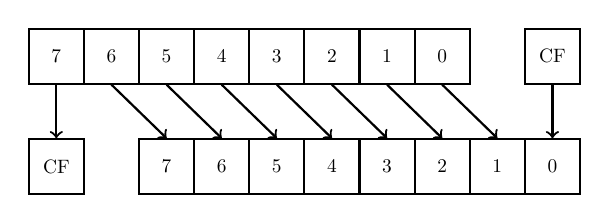
\begin{tikzpicture}[scale=0.7, every node/.style={scale=0.7}]
	\edef\bitsize{1cm}
	\tikzstyle{byte}=[draw,minimum size=\bitsize]	
	\tikzstyle{every path}=[thick]
	
	\node [draw,rectangle,minimum size=\bitsize] (a1) {7};
	\node [draw,rectangle,minimum size=\bitsize] (a2) [right of=a1] {6};
	\node [draw,rectangle,minimum size=\bitsize] (a3) [right of=a2] {5};
	\node [draw,rectangle,minimum size=\bitsize] (a4) [right of=a3] {4};
	\node [draw,rectangle,minimum size=\bitsize] (a5) [right of=a4] {3};
	\node [draw,rectangle,minimum size=\bitsize] (a6) [right of=a5] {2};
	\node [draw,rectangle,minimum size=\bitsize] (a7) [right of=a6] {1};
	\node [draw,rectangle,minimum size=\bitsize] (a8) [right of=a7] {0};
	\node (empty1) [right of=a8] {};
	\node [rectangle,draw,minimum size=\bitsize] (acf) [right of=empty1] {CF};
	
	\node (empty) [below of=a1] {};

	\node [rectangle,draw,minimum size=\bitsize] (bcf) [below of=empty] {CF};
	\node (empty2) [right of=bcf] {};
	\node [draw,rectangle,minimum size=\bitsize] (b1) [right of=empty2] {7};
	\node [draw,rectangle,minimum size=\bitsize] (b2) [right of=b1] {6};
	\node [draw,rectangle,minimum size=\bitsize] (b3) [right of=b2] {5};
	\node [draw,rectangle,minimum size=\bitsize] (b4) [right of=b3] {4};
	\node [draw,rectangle,minimum size=\bitsize] (b5) [right of=b4] {3};
	\node [draw,rectangle,minimum size=\bitsize] (b6) [right of=b5] {2};
	\node [draw,rectangle,minimum size=\bitsize] (b7) [right of=b6] {1};
	\node [draw,rectangle,minimum size=\bitsize] (b8) [right of=b7] {0};
	
	\draw [->] (a1.south) -- (bcf.north); % 7
	\draw [->] (a2.south) -- (b1.north); % 6
	\draw [->] (a3.south) -- (b2.north);
	\draw [->] (a4.south) -- (b3.north);
	\draw [->] (a5.south) -- (b4.north);
	\draw [->] (a6.south) -- (b5.north);
	\draw [->] (a7.south) -- (b6.north);
	\draw [->] (a8.south) -- (b7.north);
	\draw [->] (acf.south) -- (b8.north);

	\end{tikzpicture}
\end{center}

  \item[RCR] (M) \RU{вращать биты направо через флаг CF}\EN{rotate right via CF flag}:

\begin{center}
	\begin{tikzpicture}[scale=0.7, every node/.style={scale=0.7}]
	\edef\bitsize{1cm}
	\tikzstyle{byte}=[draw,minimum size=\bitsize]	
	\tikzstyle{every path}=[thick]

	\node [rectangle,draw,minimum size=\bitsize] (acf) {CF};
	\node (empty1) [right of=acf] {};
	
	\node [draw,rectangle,minimum size=\bitsize] (a1) [right of=empty1] {7};
	\node [draw,rectangle,minimum size=\bitsize] (a2) [right of=a1] {6};
	\node [draw,rectangle,minimum size=\bitsize] (a3) [right of=a2] {5};
	\node [draw,rectangle,minimum size=\bitsize] (a4) [right of=a3] {4};
	\node [draw,rectangle,minimum size=\bitsize] (a5) [right of=a4] {3};
	\node [draw,rectangle,minimum size=\bitsize] (a6) [right of=a5] {2};
	\node [draw,rectangle,minimum size=\bitsize] (a7) [right of=a6] {1};
	\node [draw,rectangle,minimum size=\bitsize] (a8) [right of=a7] {0};
	
	\node (empty) [below of=a1] {};

	\node [draw,rectangle,minimum size=\bitsize] (b1) [below of=empty] {7};
	\node [draw,rectangle,minimum size=\bitsize] (b2) [right of=b1] {6};
	\node [draw,rectangle,minimum size=\bitsize] (b3) [right of=b2] {5};
	\node [draw,rectangle,minimum size=\bitsize] (b4) [right of=b3] {4};
	\node [draw,rectangle,minimum size=\bitsize] (b5) [right of=b4] {3};
	\node [draw,rectangle,minimum size=\bitsize] (b6) [right of=b5] {2};
	\node [draw,rectangle,minimum size=\bitsize] (b7) [right of=b6] {1};
	\node [draw,rectangle,minimum size=\bitsize] (b8) [right of=b7] {0};
	
	\node (empty2) [right of=b7] {};
	
	\node [rectangle,draw,minimum size=\bitsize] (bcf) [right=of empty2] {CF};
	
	\draw [->] (acf.south) -- (b1.north);
	\draw [->] (a1.south) -- (b2.north);
	\draw [->] (a2.south) -- (b3.north);
	\draw [->] (a3.south) -- (b4.north);
	\draw [->] (a4.south) -- (b5.north);
	\draw [->] (a5.south) -- (b6.north);
	\draw [->] (a6.south) -- (b7.north);
	\draw [->] (a7.south) -- (b8.north);
	\draw [->] (a8.south) -- (bcf.north);

	\end{tikzpicture}
\end{center}


\index{x86!\Instructions!ROL}
\index{x86!\Instructions!ROR}
\item[ROL/ROR] (M) \IFRU{циклический сдвиг}{cyclic shift}
  
ROL: \IFRU{вращать налево}{rotate left}:

\begin{center}
	\begin{tikzpicture}[scale=0.7, every node/.style={scale=0.7}]
	\edef\bitsize{1cm}
	\tikzstyle{byte}=[draw,minimum size=\bitsize]	
	\tikzstyle{every path}=[thick]

	\node [draw,rectangle,minimum size=\bitsize] (a1) {7};
	\node [draw,rectangle,minimum size=\bitsize] (a2) [right of=a1] {6};
	\node [draw,rectangle,minimum size=\bitsize] (a3) [right of=a2] {5};
	\node [draw,rectangle,minimum size=\bitsize] (a4) [right of=a3] {4};
	\node [draw,rectangle,minimum size=\bitsize] (a5) [right of=a4] {3};
	\node [draw,rectangle,minimum size=\bitsize] (a6) [right of=a5] {2};
	\node [draw,rectangle,minimum size=\bitsize] (a7) [right of=a6] {1};
	\node [draw,rectangle,minimum size=\bitsize] (a8) [right of=a7] {0};

	\node (empty) [below of=a1] {};

	\node [draw,rectangle,minimum size=\bitsize] (b1) [below of=empty] {7};
	\node [draw,rectangle,minimum size=\bitsize] (b2) [right of=b1] {6};
	\node [draw,rectangle,minimum size=\bitsize] (b3) [right of=b2] {5};
	\node [draw,rectangle,minimum size=\bitsize] (b4) [right of=b3] {4};
	\node [draw,rectangle,minimum size=\bitsize] (b5) [right of=b4] {3};
	\node [draw,rectangle,minimum size=\bitsize] (b6) [right of=b5] {2};
	\node [draw,rectangle,minimum size=\bitsize] (b7) [right of=b6] {1};
	\node [draw,rectangle,minimum size=\bitsize] (b8) [right of=b7] {0};
	
	\node [shape=rectangle,draw,minimum size=\bitsize] (cf) [left=of b1] {CF};
	
	\draw [->] (a1.south) -- (b8.north);
	\draw [->] (a2.south) -- (b1.north);
	\draw [->] (a3.south) -- (b2.north);
	\draw [->] (a4.south) -- (b3.north);
	\draw [->] (a5.south) -- (b4.north);
	\draw [->] (a6.south) -- (b5.north);
	\draw [->] (a7.south) -- (b6.north);
	\draw [->] (a8.south) -- (b7.north);
	
	\draw [->] (a1.south) -- (cf.north);

	\end{tikzpicture}
\end{center}



ROR: \IFRU{вращать направо}{rotate right}:

\begin{center}
	\begin{tikzpicture}[scale=0.7, every node/.style={scale=0.7}]
	\edef\bitsize{1cm}
	\tikzstyle{byte}=[draw,minimum size=\bitsize]	
	\tikzstyle{every path}=[thick]

	\node [draw,rectangle,minimum size=\bitsize] (a1) {7};
	\node [draw,rectangle,minimum size=\bitsize] (a2) [right of=a1] {6};
	\node [draw,rectangle,minimum size=\bitsize] (a3) [right of=a2] {5};
	\node [draw,rectangle,minimum size=\bitsize] (a4) [right of=a3] {4};
	\node [draw,rectangle,minimum size=\bitsize] (a5) [right of=a4] {3};
	\node [draw,rectangle,minimum size=\bitsize] (a6) [right of=a5] {2};
	\node [draw,rectangle,minimum size=\bitsize] (a7) [right of=a6] {1};
	\node [draw,rectangle,minimum size=\bitsize] (a8) [right of=a7] {0};

	\node (empty) [below of=a1] {};

	\node [draw,rectangle,minimum size=\bitsize] (b1) [below of=empty] {7};
	\node [draw,rectangle,minimum size=\bitsize] (b2) [right of=b1] {6};
	\node [draw,rectangle,minimum size=\bitsize] (b3) [right of=b2] {5};
	\node [draw,rectangle,minimum size=\bitsize] (b4) [right of=b3] {4};
	\node [draw,rectangle,minimum size=\bitsize] (b5) [right of=b4] {3};
	\node [draw,rectangle,minimum size=\bitsize] (b6) [right of=b5] {2};
	\node [draw,rectangle,minimum size=\bitsize] (b7) [right of=b6] {1};
	\node [draw,rectangle,minimum size=\bitsize] (b8) [right of=b7] {0};
	
	\node [shape=rectangle,draw,minimum size=\bitsize] (cf) [right=of b7] {CF};
	
	\draw [->] (a1.south) -- (b2.north);
	\draw [->] (a2.south) -- (b3.north);
	\draw [->] (a3.south) -- (b4.north);
	\draw [->] (a4.south) -- (b5.north);
	\draw [->] (a5.south) -- (b6.north);
	\draw [->] (a6.south) -- (b7.north);
	\draw [->] (a7.south) -- (b8.north);
	\draw [->] (a8.south) -- (b1.north);
	
	\draw [->] (a8.south) -- (cf.north);

	\end{tikzpicture}
\end{center}



\IFRU{Не смотря на то что многие \ac{CPU} имеют эти инструкции, в \CCpp нет соответствующих операций,
так что компиляторы с этих \ac{PL} обычно не генерируют код использующий эти инструкции}{Despite the 
fact that almost all \ac{CPU}s has these instructions, there are no corresponding
operations in the \CCpp, so the compilers of these \ac{PL}s are usually not generating these 
instructions}.

\IFRU{Чтобы программисту были доступны эти инструкции, в \ac{MSVC} есть псевдофункции}
{For programmer's convenience, at least \ac{MSVC} has pseudofunctions} (compiler intrinsics)
\IT{\_rotl()} \AndENRU \IT{\_rotr()}\FNMSDNROTxURL{},
\IFRU{которые транслируются компилятором напрямую в эти инструкции}
{which are translated by compiler directly to these instructions}.


\index{x86!\Instructions!SAL}
  \item[SAL] \RU{Арифметический сдвиг влево}\EN{Arithmetic shift left}, \RU{синонимично}\EN{synonymous to} \TT{SHL}

\index{x86!\Instructions!SAR}
  \label{ins:SAR}
  \item[SAR] \RU{Арифметический сдвиг вправо}\EN{Arithmetic shift right}

\begin{center}
	\begin{tikzpicture}[scale=0.7, every node/.style={scale=0.7}]
	\edef\bitsize{1cm}
	\tikzstyle{byte}=[draw,minimum size=\bitsize]	
	\tikzstyle{every path}=[thick]

	\node [draw,rectangle,minimum size=\bitsize] (a1) {7};
	\node [draw,rectangle,minimum size=\bitsize] (a2) [right of=a1] {6};
	\node [draw,rectangle,minimum size=\bitsize] (a3) [right of=a2] {5};
	\node [draw,rectangle,minimum size=\bitsize] (a4) [right of=a3] {4};
	\node [draw,rectangle,minimum size=\bitsize] (a5) [right of=a4] {3};
	\node [draw,rectangle,minimum size=\bitsize] (a6) [right of=a5] {2};
	\node [draw,rectangle,minimum size=\bitsize] (a7) [right of=a6] {1};
	\node [draw,rectangle,minimum size=\bitsize] (a8) [right of=a7] {0};

	\node (empty) [below of=a1] {};

	\node [draw,rectangle,minimum size=\bitsize] (b1) [below of=empty] {7};
	\node [draw,rectangle,minimum size=\bitsize] (b2) [right of=b1] {6};
	\node [draw,rectangle,minimum size=\bitsize] (b3) [right of=b2] {5};
	\node [draw,rectangle,minimum size=\bitsize] (b4) [right of=b3] {4};
	\node [draw,rectangle,minimum size=\bitsize] (b5) [right of=b4] {3};
	\node [draw,rectangle,minimum size=\bitsize] (b6) [right of=b5] {2};
	\node [draw,rectangle,minimum size=\bitsize] (b7) [right of=b6] {1};
	\node [draw,rectangle,minimum size=\bitsize] (b8) [right of=b7] {0};
	
	\node [shape=rectangle,draw,minimum size=\bitsize] (cf) [right=of b7] {CF};
	
	\draw [->] (a1.south) -- (b1.north); %7
	\draw [->] (a1.south) -- (b2.north); %6

	\draw [->] (a2.south) -- (b3.north); %6
	\draw [->] (a3.south) -- (b4.north); %5
	\draw [->] (a4.south) -- (b5.north); %4
	\draw [->] (a5.south) -- (b6.north); %3
	\draw [->] (a6.south) -- (b7.north); %2
	\draw [->] (a7.south) -- (b8.north); %1
	
	\draw [->] (a8.south) -- (cf.north);

	\end{tikzpicture}
\end{center}

\RU{Таким образом, бит знака всегда остается на месте}
\EN{Hence, the sign bit always stays at the place of the} \ac{MSB}.


\myindex{x86!\Instructions!SETcc}
  \item[SETcc] op: \RU{загрузить 1 в op (только байт) если условие верно или 0 если наоборот}
  \EN{load 1 to operand (byte only) if the condition is true or zero otherwise}.
  \RU{Коды точно такие же, как и в инструкциях Jcc}\EN{The condition codes are the same as in the Jcc instructions} 
  (\myref{Jcc}).


\index{x86!\Instructions!STC}
\index{x86!\Flags!CF}
  \item[STC] (M) \RU{установить флаг CF}\EN{set CF flag}

\index{x86!\Instructions!STD}
\index{x86!\Flags!DF}
  \item[STD] (M) \RU{установить флаг DF}\EN{set DF flag}.
   \RU{Эта инструкция не генерируется компиляторами и вообще редкая.}
   \EN{This instruction is not generated by compilers and generally rare.}
   \RU{Например, она может быть найдена в файле}\EN{For example, it can be found in the} 
   \TT{ntoskrnl.exe} \RU{(ядро Windows) в написанных вручную функциях копирования 
   памяти}\EN{Windows kernel file, in the hand-written memory copy routines}.

\index{x86!\Instructions!STI}
\index{x86!\Flags!IF}
  \item[STI] (M) \RU{установить флаг IF}\EN{set IF flag}

\index{x86!\Instructions!SYSCALL}
  \item[SYSCALL] (AMD) \IFRU{вызов сисколла}{call syscall} (\ref{syscalls})

\index{x86!\Instructions!SYSENTER}
  \item[SYSENTER] (Intel) \IFRU{вызов сисколла}{call syscall} (\ref{syscalls})

\myindex{x86!\Instructions!UD2}
  \item[UD2] (M) \RU{неопределенная инструкция, вызывает исключение. Применяется для тестирования.}
  \EN{undefined instruction, raises exception. Used for testing.}

\end{description}

\subsubsection{\IFRU{Инструкции FPU}{FPU instructions}}

\IFRU{-R в названии инструкции обычно означает что операнды поменены местами, -P означает
что один элемент выталкивается из стека после исполнения инструкции, -PP означает что
выталкиваются два элемента}
{-R in mnemonic usually means that operands are reversed, -P means that one element is popped
from the stack after instruction execution, -PP means that two elements are popped}.

-P \IFRU{инструкции часто бывают полезны, когда нам уже больше не нужно хранить значение в FPU-стеке}
{instructions are often useful when we do not need a value in the FPU stack to be present anymore}.

\begin{description}
\index{x86!\Instructions!FABS}
  \item[FABS] \IFRU{заменить значение в ST(0) на абсолютное значение ST(0)}{replace value in ST(0) by absolute value in ST(0)}

\index{x86!\Instructions!FADD}
\index{x86!\Instructions!FADDP}
  \item[FADD] op: ST(0)=op+ST(0)
  \item[FADD] ST(0), ST(i): ST(0)=ST(0)+ST(i)
  \item[FADDP] ST(1)=ST(0)+ST(1);
  \RU{вытолкнуть один элемент из стека, таким образом, складываемые значения в стеке заменяются
  суммой}\EN{pop one element from the stack, i.e., the values in the stack are replaced by their sum}

 % + FADDP
\index{x86!\Instructions!FCHS}
  \item[FCHS]: ST(0)=-ST(0)


\index{x86!\Instructions!FCOM}
\index{x86!\Instructions!FCOMP}
\index{x86!\Instructions!FCOMPP}
  \item[FCOM] \IFRU{сравнить}{compare} ST(0) \IFRU{с}{with} ST(1)
  \item[FCOM] op: \IFRU{сравнить}{compare} ST(0) \IFRU{с}{with} op
  \item[FCOMP] \IFRU{сравнить}{compare} ST(0) \IFRU{с}{with} ST(1); \IFRU{вытолкнуть один элемент из стека}
  {pop one element from the stack}
  \item[FCOMPP] \IFRU{сравнить}{compare} ST(0) \IFRU{с}{with} ST(1); \IFRU{вытолкнуть два элемента из стека}
  {pop two elements from the stack}

 % + FCOMP + FCOMPP
\myindex{x86!\Instructions!FDIVR}
\myindex{x86!\Instructions!FDIVRP}
  \item[FDIVR] op: ST(0)=op/ST(0)
  \item[FDIVR] ST(i), ST(j): ST(i)=ST(j)/ST(i)
  \item[FDIVRP] op: ST(0)=op/ST(0); \RU{вытолкнуть один элемент из стека}\EN{pop one element from the stack}
  \item[FDIVRP] ST(i), ST(j): ST(i)=ST(j)/ST(i); \RU{вытолкнуть один элемент из стека}\EN{pop one element from the stack}


 % + FDIVRP
\index{x86!\Instructions!FDIV}
\index{x86!\Instructions!FDIVP}
  \item[FDIV] op: ST(0)=ST(0)/op
  \item[FDIV] ST(i), ST(j): ST(i)=ST(i)/ST(j)
  \item[FDIVP] ST(1)=ST(0)/ST(1); \RU{вытолкнуть один элемент из стека, таким образом, 
  делимое и делитель в стеке заменяются частным}\EN{pop one element from the stack, i.e., 
  dividend and divisor values in the stack are replaced by quotient}
 % + FDIVP
\index{x86!\Instructions!FILD}
  \item[FILD] op: \RU{сконвертировать целочисленный op и затолкнуть его в стек}
  \EN{convert integer and push it to the stack}.


\index{x86!\Instructions!FIST}
\index{x86!\Instructions!FISTP}
  \item[FIST] op: \RU{конвертировать}\EN{convert} ST(0) \RU{в целочисленное}\EN{to integer} op
  \item[FISTP] op: \RU{конвертировать}\EN{convert} ST(0) \RU{в целочисленное}\EN{to integer} op; 
  \RU{вытолкнуть один элемент из стека}\EN{pop one element from the stack}
 % + FISTP
\myindex{x86!\Instructions!FLD1}
  \item[FLD1] \RU{затолкнуть 1 в стек}\EN{push 1 to stack}


\index{x86!\Instructions!FLDCW}
  \item[FLDCW] op: \IFRU{загрузить}{load} FPU control word (\ref{FPU_control_word}) \IFRU{из}{from} 16-bit op.


\index{x86!\Instructions!FLDZ}
  \item[FLDZ] \IFRU{затолкнуть ноль в стек}{push zero to stack}



\index{x86!\Instructions!FLD}
  \item[FLD] op: \IFRU{затолкнуть op в стек}{push op to the stack}.

\index{x86!\Instructions!FMUL}
\index{x86!\Instructions!FMULP}
  \item[FMUL] op: ST(0)=ST(0)*op
  \item[FMUL] ST(i), ST(j): ST(i)=ST(i)*ST(j)
  \item[FMULP] op: ST(0)=ST(0)*op; \IFRU{вытолкнуть один элемент из стека}{pop one element from the stack}
  \item[FMULP] ST(i), ST(j): ST(i)=ST(i)*ST(j); \IFRU{вытолкнуть один элемент из стека}{pop one element from the stack}

 % + FMULP
\myindex{x86!\Instructions!FSINCOS}
  \item[FSINCOS]: tmp=ST(0); ST(1)=sin(tmp); ST(0)=cos(tmp)


\myindex{x86!\Instructions!FSQRT}
  \item[FSQRT]: $ST(0)=\sqrt{ST(0)}$


\index{x86!\Instructions!FSTCW}
\index{x86!\Instructions!FNSTCW}
  \item[FSTCW] op: \RU{записать}\EN{store} FPU control word (\ref{FPU_control_word}) \RU{в}\EN{into} 16-bit op
  \RU{после проверки ожидающих исключений}\EN{after checking for pending exceptions}.
  \item[FNSTCW] op: \RU{записать}\EN{store} FPU control word (\ref{FPU_control_word}) \RU{в}\EN{into} 16-bit op.

 % + FNSTCW
\index{x86!\Instructions!FSTSW}
\index{x86!\Instructions!FNSTSW}
  \item[FSTSW] op: \RU{записать}\EN{store} FPU status word (\myref{FPU_status_word}) \RU{в}\EN{into} 16-bit op
  \RU{после проверки ожидающих исключений}\EN{after checking for pending exceptions}.
  \item[FNSTSW] op: \RU{записать}\EN{store} FPU status word (\myref{FPU_status_word}) \RU{в}\EN{into} 16-bit op.

 % + FNSTSW
\index{x86!\Instructions!FST}
\index{x86!\Instructions!FSTP}
  \item[FST] op: \IFRU{копировать}{copy} ST(0) \IFRU{в}{to} op
  \item[FSTP] op: \IFRU{копировать}{copy} ST(0) \IFRU{в}{to} op; \IFRU{вытолкнуть один элемент из стека}
  {pop one element from the stack}

\index{x86!\Instructions!FSUBR}
\index{x86!\Instructions!FSUBRP}
  \item[FSUBR] op: ST(0)=op-ST(0)
  \item[FSUBR] ST(0), ST(i): ST(0)=ST(i)-ST(0)
  \item[FSUBRP] ST(1)=ST(0)-ST(1);
  \RU{вытолкнуть один элемент из стека, таким образом, складываемые значения в стеке заменяются
  разностью}\EN{pop one element from the stack, i.e., the value in the stack is replaced by the difference}

 % + FSUBRP
\index{x86!\Instructions!FSUB}
\index{x86!\Instructions!FSUBP}
  \item[FSUB] op: ST(0)=ST(0)-op
  \item[FSUB] ST(0), ST(i): ST(0)=ST(0)-ST(i)
  \item[FSUBP] ST(1)=ST(1)-ST(0);
  \RU{вытолкнуть один элемент из стека, таким образом, складываемые значения в стеке заменяются
  разностью}\EN{pop one element from the stack, i.e., summed values in the stack are replaced by difference}

 % + FSUBP
\index{x86!\Instructions!FUCOM}
\index{x86!\Instructions!FUCOMP}
\index{x86!\Instructions!FUCOMPP}
  \item[FUCOM] ST(i): \RU{сравнить}\EN{compare} ST(0) \AndENRU ST(i)
  \item[FUCOM]: \RU{сравнить}\EN{compare} ST(0) \AndENRU ST(1)
  \item[FUCOMP]: \RU{сравнить}\EN{compare} ST(0) \AndENRU ST(1); \RU{вытолкнуть один элемент из стека}\EN{pop one element from stack}.
  \item[FUCOMPP]: \RU{сравнить}\EN{compare} ST(0) \AndENRU ST(1); \RU{вытолкнуть два элемента из стека}\EN{pop two elements from stack}.
 
  \RU{Инструкция работает так же, как и FCOM, за тем исключением что исключение срабатывает только
  если один из операндов SNaN, но числа QNaN нормально обрабатываются}\EN{The instructions performs just like FCOM, but exception is raised only if one of operands is SNaN,
  while QNaN numbers are processed smoothly}.
 % + FUCOMP + FUCOMPP
\index{x86!\Instructions!FXCH}
  \item[FXCH] ST(i) \RU{обменять местами значения в ST(0) и ST(i)}\EN{exchange values in ST(0) and ST(i)}
  \item[FXCH] \RU{обменять местами значения в ST(0) и ST(1)}\EN{exchange values in ST(0) and ST(1)}


\end{description}

\subsubsection{\IFRU{SIMD-инструкции}{SIMD instructions}}

% TODO

%\begin{description}
%\input{appendix/x86/instructions/DIVSD}
%\input{appendix/x86/instructions/MOVDQA}
%\input{appendix/x86/instructions/MOVDQU}
%\input{appendix/x86/instructions/PADDD}
%\input{appendix/x86/instructions/PCMPEQB}
%\input{appendix/x86/instructions/PLMULHW}
%\input{appendix/x86/instructions/PLMULLD}
%\input{appendix/x86/instructions/PMOVMSKB}
%\input{appendix/x86/instructions/PXOR}
%\end{description}

% SHLD !
% SHRD !
% BSWAP !
% CMPXCHG
% XADD !
% CMPXCHG8B
% RDTSC !
% PAUSE!

% xsave
% fnclex, fnsave
% movsxd, movaps, wait, sfence, lfence, pushfq
% prefetchw
% REP RETN
% REP BSF
% movnti, movntdq, rdmsr, wrmsr
% ldmxcsr, stmxcsr, invlpg
% swapgs
% movq, movd
% mulsd
% POR
% IRETQ
% pslldq
% psrldq
% cqo, fxrstor, comisd, xrstor, wbinvd, movntq
% fprem
% addsb, subsd, frndint

% rare:
%\item[ENTER]
%\item[LEAVE]
%\item[LES]
% LDS
% XLAT

 % subsection
